\documentclass[a4paper,12pt]{article}

\usepackage[english,brazil]{babel}
\usepackage[utf8]{inputenc}
\usepackage{icomma}
\usepackage{amsmath}
\usepackage{makecell}
\usepackage{graphicx}
\usepackage{fancyhdr}
\usepackage{url}
\renewcommand{\baselinestretch}{1.5}
\usepackage{titling}
\usepackage{geometry}
\usepackage{subfigure}
\geometry{
 a4paper,
 left=35mm,
 right=15mm,
 top=1in,
 bottom=1in,
}
\usepackage{amsmath}
\usepackage{amssymb}
\usepackage{subfigure}
\usepackage{multirow}
\usepackage[table]{xcolor}
\usepackage[backend=bibtex,style=ieee,sorting=none]{biblatex}
\usepackage{algorithm}
\usepackage[noend]{algpseudocode}
\usepackage{pdfpages}
\usepackage{enumerate}
\bibliography{main}
\newcolumntype{C}{>{\centering\arraybackslash}p{1em}}


\newpage

\begin{document}
\selectlanguage{brazil}

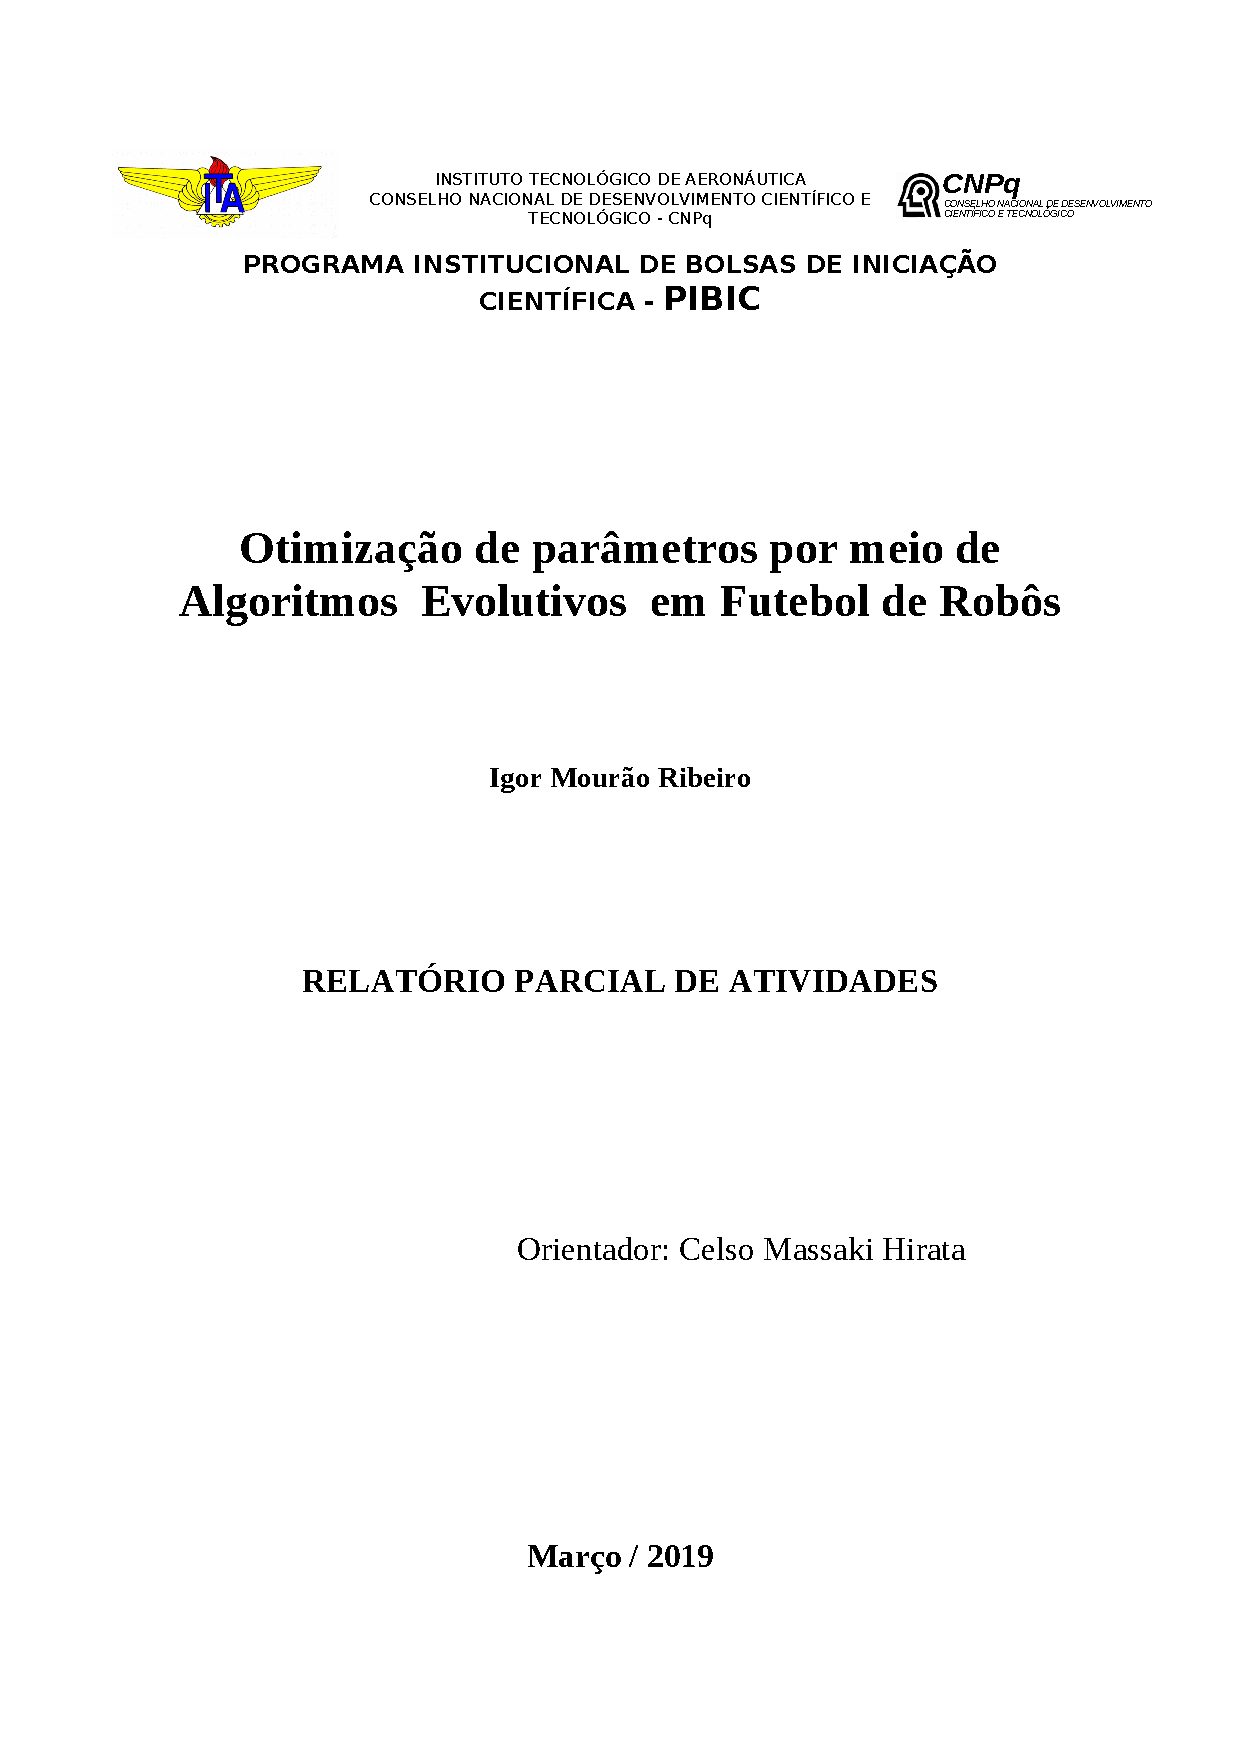
\includepdf[pages={1-},scale=1]{Inicio.pdf}


\tableofcontents

\newpage

\section{Resumo do Plano Inicial}
\label{secao:plano_inicial}

O objetivo deste trabalho é desenvolver e implementar um algoritmo para a otimização de parâmetros de um time composto por três robôs diferenciais. O contexto é uma partida de futebol segundo a Competição Brasileira de Robótica (CBR), categoria IEEE Very Small Size Soccer (VSSS). Por meio da criação de métricas e testes automatizados para medir o desempenho do time de robôs em diversas situações de jogo, pode-se utilizar algoritmos evolutivos para fazer a otimização de parâmetros relevantes, como os relativos ao planejamento de trajetória. Visa-se utilizar os algoritmos aqui implementados pela equipe da ITAndroids, que representa o ITA em competições nacionais e internacionais, como na competição Latin America Robotics Competition (LARC)/CBR.

Planejamento:
\begin{itemize}

\item 1o Bimestre (ago / set): Estudo da literatura e revisão bibliográfica sobre o tema de otimização de parâmetros para robôs jogadores de futebol.

\item 2o Bimestre (out / nov): Seleção de métricas a serem utilizadas e implementação inicial do código.

\item 3o Bimestre (dez / jan): Implementação dos testes e simulações para as métricas escolhidas. Redação do relatório parcial.

\item 4o Bimestre (fev / mar): Análise e implementação do algoritmo escolhido.

\item 5o Bimestre (abr / mai): Análise do desempenho da otimização para o planejamento de trajetórias. Ajuste do algoritmo para melhores resultados.

\item 6o Bimestre (jun / jul): Redação do relatório final. Redação do artigo para o ENCITA. Teste final para o software completo no robô real, com todas as áreas do projeto operantes.

\end{itemize}

\section{Resumo das Atividades Realizadas}
\label{secao:atividades_realizadas}

Ao longo dos dois primeiros meses, foram realizados estudos e foi decidido que será usado o algoritmo Covariance Matrix Adaptation Evolution Strategy (CMA-ES) para a otimização de parâmetros. Esse algoritmo foi escolhido dentre de opções como Particle Swarm Optimization (PSO) e o Algoritmo Genético. Mais detalhes sobre esses dois últimos métodos pode ser encontrada, respectivamente, em \cite{PSO} e em \cite{genetico}. Para uma descrição sobre a eficácia do algoritmo CMA-ES no contexto de futebol de robôs, pode-se encontrar na referência \cite{CMA-ES-Soccer}.

Ao longo do segundo e terceiro bimestres, a base do algoritmo foi implementada utilizando Matlab \cite{matlab}, que é uma linguagem especializada em algébra linear utilizada pela equipe. Foi, em seguida, realizada a escolha e codificação das métricas a serem utilizadas para medir o desempenho de uma determinada situação de jogo.

O algoritmo foi, em seguida, implementado e integrado com o restante do código da equipe. Após algumas iterações, os parâmetros relativos ao planejamento de trajetória do robô foram otimizados e testados em simulações. Os resultados se mostraram satisfatórios e condizentes com o previsto. Ressalta-se que apenas alguns parâmetros precisaram de algum ajuste ao serem implementados no robô real, de forma que grande parte do trabalho de otimizar parâmetros manualmente foi poupada.

Os resultados obtidos foram efetivos como mostrado na LARC, ocorrida entre os dias 6 a 10 de novembro de 2018. O algoritmo mostrou que o planejamento de trajetórias da equipe, em conjunto com o controle do robô, estavam muito precisos, fato que concedeu à equipe uma vantagem decisiva na competição. A equipe da ITAndroids conquistou o primeiro lugar da competição, sendo a sua classificação a mais alta  na categoria Very Small Size Soccer na história.
\section{Descrição do Problema}
\label{secao:enunciado_problema}

No contexto do futebol de robôs, a otimização de parâmetros traz muitos desafios. Tal problema consiste no fato de se implementar um algoritmo que consiga encontrar as melhores constantes a serem usadas no código para melhorar o desempenho do robô em uma partida real. Entretando, para encontrar esses parâmetros de forma automatizada, é necessário, além do algoritmo evolutivo em si, a existência de simulações fiéis à realidade. A Figura \ref{fig:vss_ele} mostra a placa eletrônica do robô utilizado.

\begin{figure}[H]
	\centering
	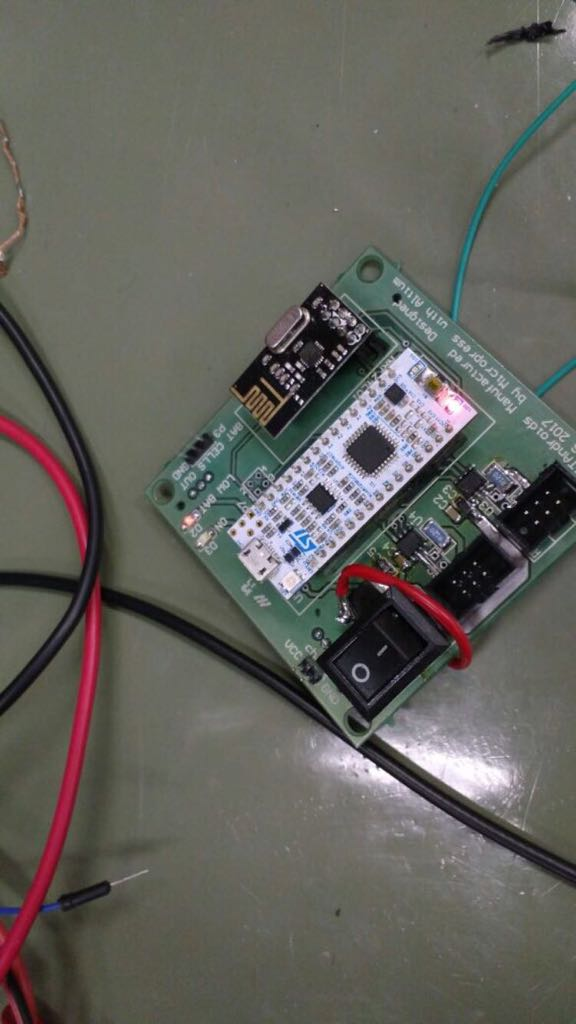
\includegraphics[width=0.5\textwidth]{figures/vss_ele.jpg}
   \caption{Placa eletrônica de um robô Very Small Size.} \label{fig:vss_ele}
\end{figure}

Nesse projeto, trabalhou-se com os robôs da competição IEEE Very Small Size (VSS): uma competição de futebol de robôs completamente automatizada em que cada robô tem como tamanho máximo um cubo de 7,5 cm de aresta. O campo de futebol possui 1,5 m de comprimento e 1,3 m de largura. Cada time tem 3 jogadores: que podem assumir posições dinâmicas, como goleiro e atacante, ao decorrer de uma partida. Uma câmera proporciona a visão aérea com as posições de todos os elementos da partida. As regras completas podem ser lidas em \cite{cbr2008}.

\begin{figure}[H]
	\centering
	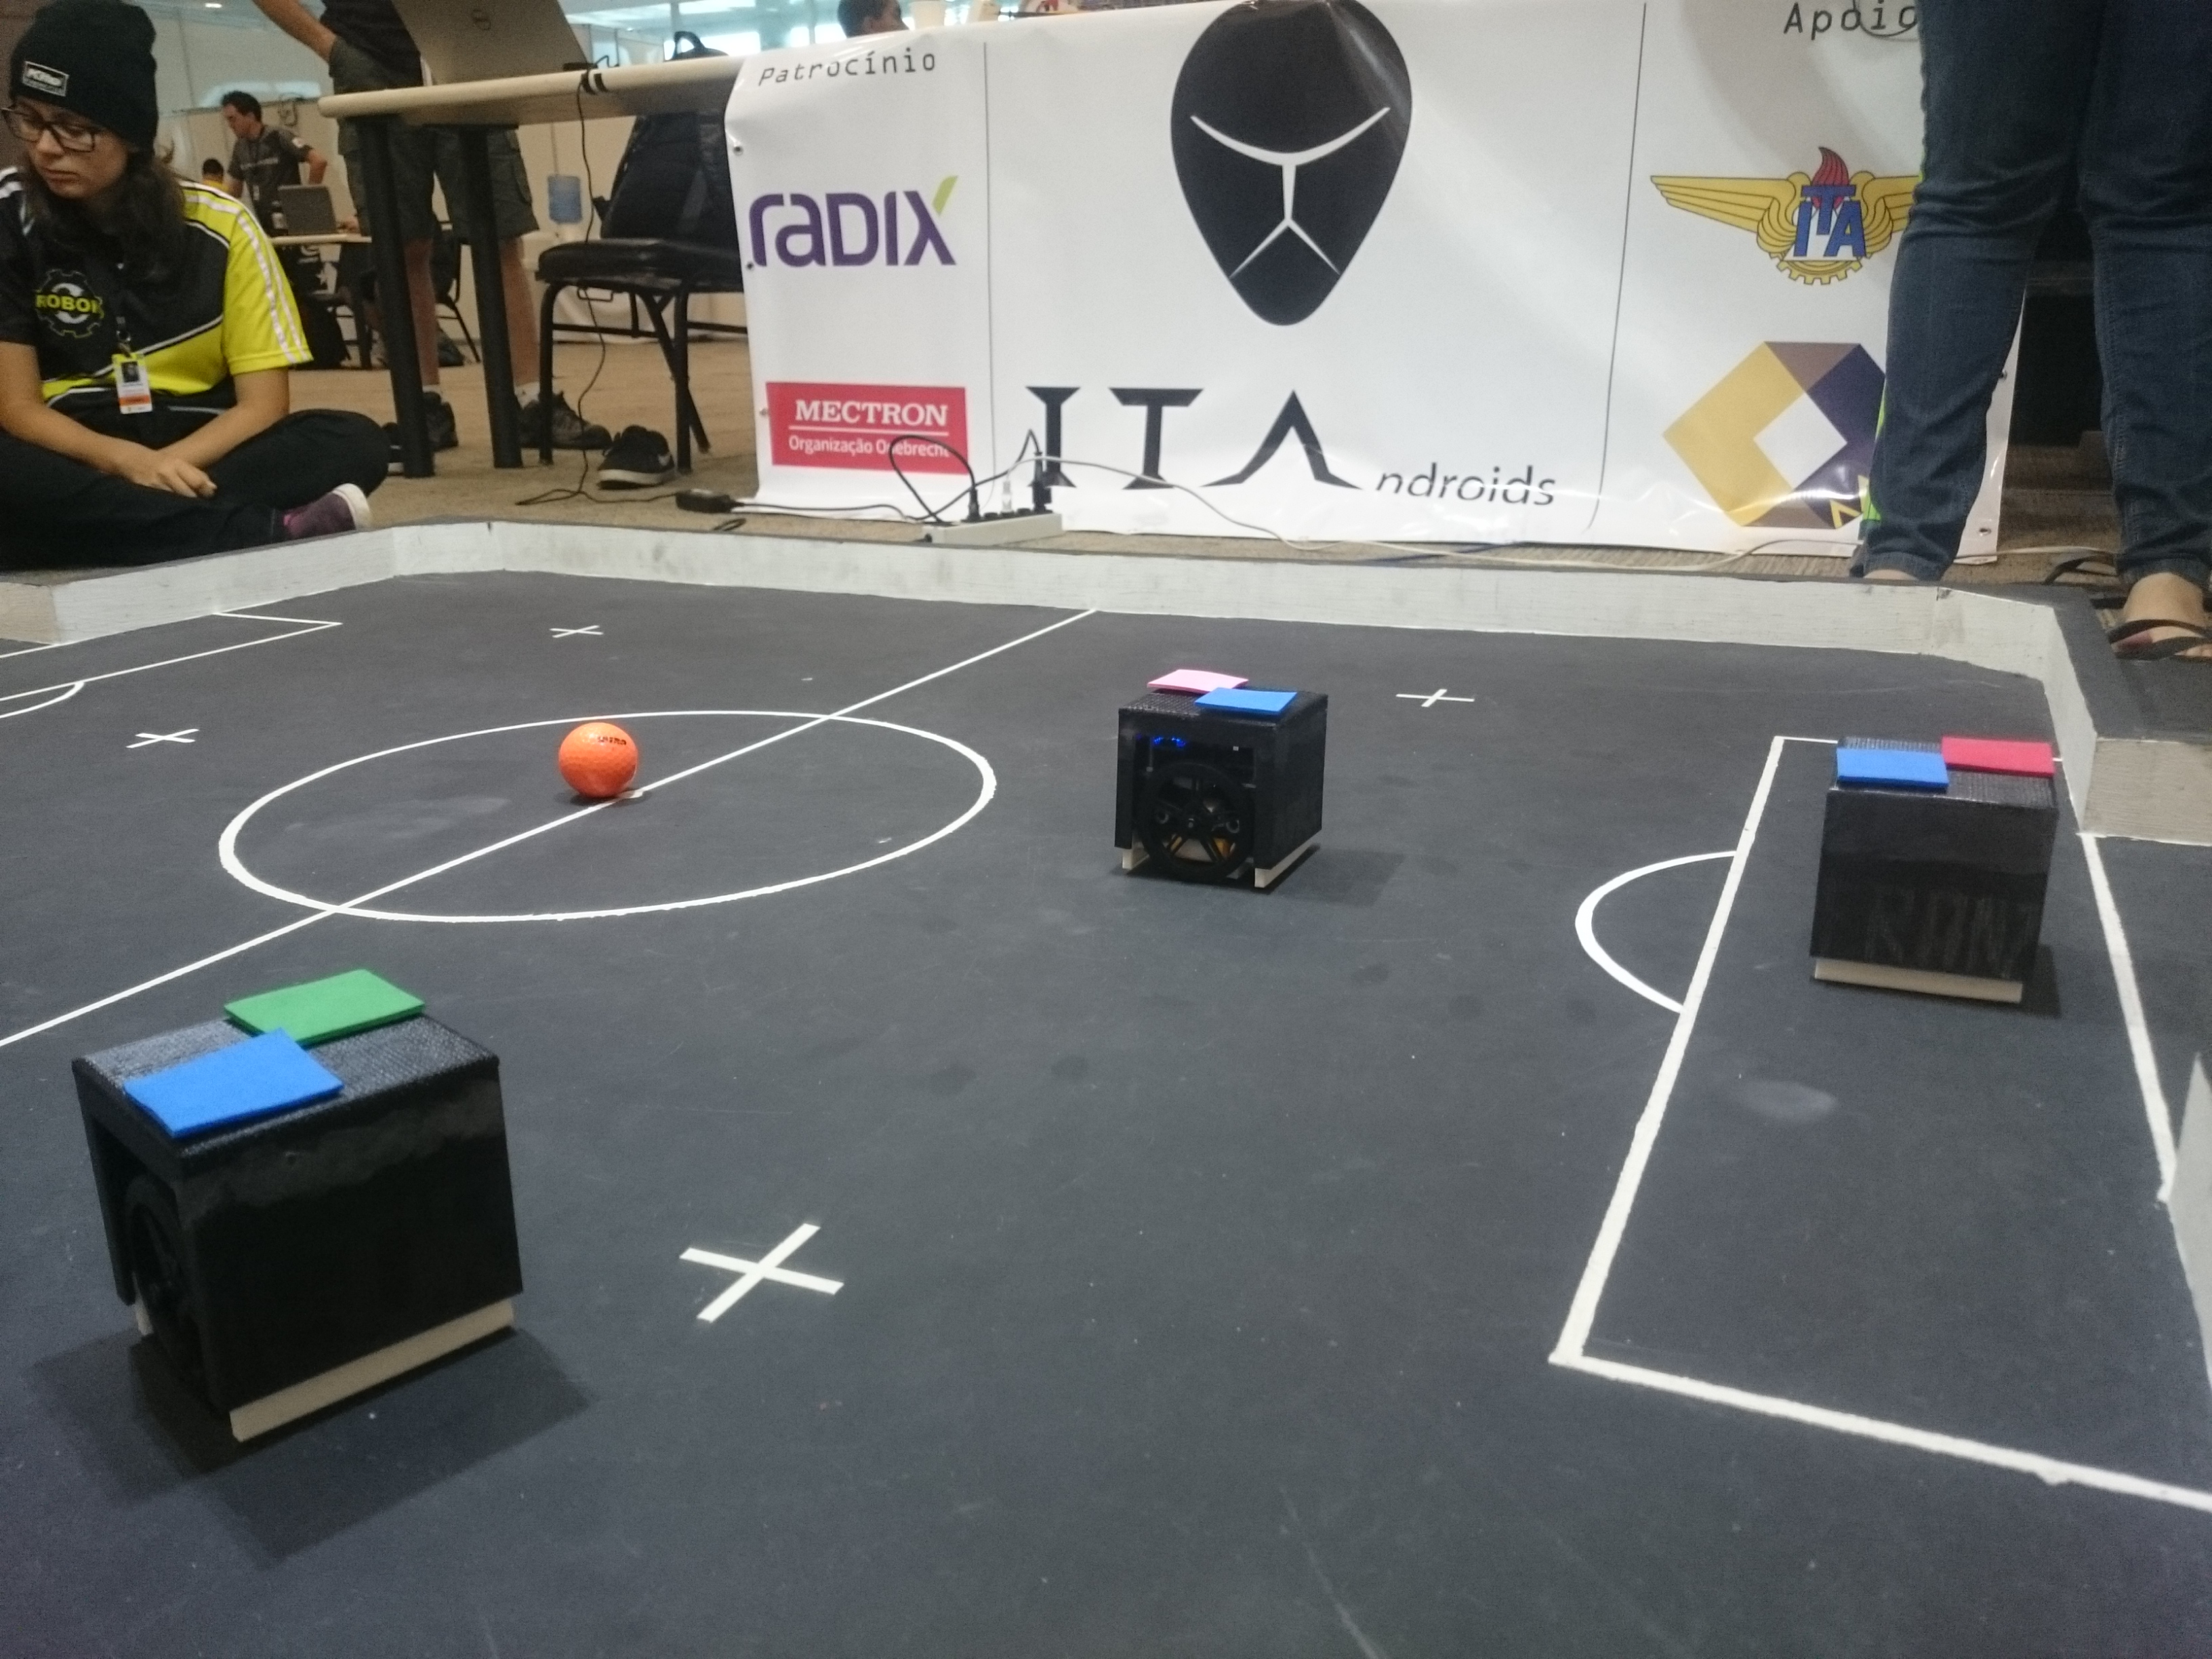
\includegraphics[width=0.5\textwidth]{figures/vss.JPG}
   \caption{Robôs da ITAndroids da categoria IEEE VSSS.} \label{fig:vss}
\end{figure}

A Figura \ref{fig:vss} mostra os robôs usados nas competições. A visão computacional utilizada pela equipe ITAndroids pode ser encontrada com mais detalhes em \cite{small_vision} e utiliza uma câmera no topo do campo que repassa informações para um computador processar, como visto na Figura \ref{fig:funcioamento}.

\begin{figure}[H]
	\centering
		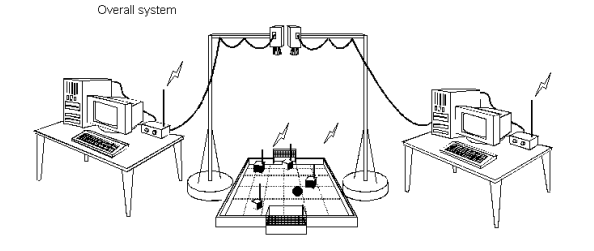
\includegraphics[width=0.7\textwidth]{figures/overview.png}
  \caption{Representação do funcionamento técnico de um jogo de VSS.}
	\label{fig:funcioamento}
\end{figure}

Cada robô foi projetado com duas rodas laterais e material teflon para diminuir atrito no deslizamento de seu chassis. Essa característica o torna um robô diferencial. Ou seja, temos o controle sobre as velocidades linear e angular, mas não é possível mover o robô para os lados. A linguagem utilizada para o projeto foi C++; diferente da utilizada nesse trabalho, que é Matlab; pois é uma linguagem que tem uma velocidade de execução alta e tem boa escalabilidade para um projeto grande. 

Nesse contexto, surgem várias questões a serem resolvidas para se ter um time vencedor. Nesse projeto, será abordado o seguinte problema de otimização: dado um simulador feito pela equipe que simula a física e a lógica de uma partida oficial, deve-se encontrar os melhores valores possíveis para as constantes do planejamento de trajetórias, de modo a maximizar o desempenho do time em uma partida com os robôs reais.

Sobre o assunto de planejamento de trajetórias, o utilizado pela equipe é o Univector Field \cite{univector}, que é muito eficiente e já demonstrou bons resultados em competições oficiais com algumas das melhores equipes utilizando-o. Uma das suas desvantagens, é a existência de sete parâmetros diferentes para serem otimizados e de que essas constantes não são intuitivas para uma pessoa ajustá-las sem ajuda de um computador. Isso acontece devido ao comportamento do algoritmo ser relativamente complexo quando comparado com outras alternativas como o algoritmo Campos Potenciais \cite{potential_fields}.

Além disso, é importante ressaltar que o tempo de execução do algoritmo deve ser o mínimo possível. Nota-se que não é possível simular uma partida completa de futebol já que isso demoraria bastante e o algoritmo precisa de em torno de 100 iterações para convergir. Para isso, técnicas para executar simulações aceleradas e executar situações específicas de jogo foram desenvolvidas, com o objetivo de reduzir o tempo total da otimização.

Ademais, outro problema que será enfrentado no desenvolvimento desse projeto é a criação de interfaces de comunicação entre o algoritmo de otimização, a ser codificado em Matlab, com o código do projeto e das simulações, ambos codificados na linguagem de programação C++.

Para resolver esse problema, foi escolhido como algoritmo para a otimização de parâmetros o Covariance Matrix Adaptation Evolution Strategy, já que ele consegue otimizar problemas não lineares e não convexos, que, devido à elevada complexidade, é o caso do futebol de robôs.

\subsection{Covariance Matrix Adaptation Evolution Strategy}

O algoritmo CMA-ES é uma estratégia evolutiva. Um algoritmo evolutivo é baseado no princípio da evolução biológica, em que conceitos de recombinação e mutação de genes são aplicados para selecionar melhores indivíduos. Mais formalmente: em cada geração novos indivíduos são criados a partir de seus pais, com o objetivo de gerar melhores indivíduos segundo algum critério.

No contexto da computação, cada geração será considerada uma iteração. Em cada iteração existirá uma população composta de indivíduos (ou candidatos) que deverá ser alterada segundo um algoritmo para diminuir uma determinada função de custo. 

Para o caso do CMA-ES, os novos indivíduos são escolhidos com base em uma distribuição gaussiana de múltiplas dimensões. A nova população será gerada a partir da média dos melhores indíviduos da população anterior, em combinação com uma perturbação gaussiana estocástica. Dependência entre diferentes parâmetros são representadas por uma matriz de covariâncias.

Nota-se que o algoritmo, brevemente descrito, não usa derivadas nem valores das funções de custo, apenas importa a comparação entre os desempenhos dos indíviduos de uma população.

\subsubsection{O algoritmo}

O algoritmo do CMA-ES pode ser separado em alguma etapas:

\begin{enumerate}
\item Escolha dos parâmetros iniciais para a otimização: o tamanho do passo, o ponto inicial, o tamanho da população e as condições de parada do algoritmo (que podem ser número de iterações ou ter um custo menor que um certo valor).
\item Enquanto a condição de parada não for atingida:
\begin{enumerate}
\item Gera novas soluções a partir da média dos melhores indivíduos da iteração anterior. Para isso usa-se uma distribuição gaussiana normal centrada em tal média e variância inicial igual ao tamanho do passo.
\item Cálculo dos custos de cada novo indivíduo por meio de uma função chamada de fitness.
\item Ordenação dos indíviduos, com base nos seus custos.
\item Atualização dos valores de variáveis internas.
\end{enumerate}
\end{enumerate}

Não será abordado os detalhes técnicos do item 2d, pois a implementação desse algoritmo não é o foco desse trabalho. Essa decisão ocorreu porque, além de tal passo ser bastante complexo estatisticamente, esse item apenas otimiza a velocidade de convergência do algoritmo e não é necessário para o entendimento inicial da estratégia evolutiva. Uma descrição mais profunda e detalhada de como otimizar o CMA-ES se encontra em \cite{CMA-ES}.

\subsection{O simulador}

Testes no robô real precisam de trabalho adicional devido a problemas que podem surgir como: bateria dos robôs acaba e precisa ser trocada, problemas no hardware ou mecânica do robô, campo sujo e necessidade de reposicionamento manual dos robôs. Por isso, a equipe ITAndroids desenvolveu um simulador próprio com o objetivo de resolver essas dificuldades.

O simulador é uma aplicação separada do código principal do time, desenvolvida e idealizada pela própria equipe, que cria um ambiente com física que simula um jogo. Tal aplicação se comunica com o código principal por meio de uma biblioteca de comunicação chamada Protocol Buffers \cite{protobuf}. Para isso, o simulador transmite informações como as posições e velocidades dos robôs para o código principal, enquanto que esse último transmite informações de velocidade das rodas de cada robô para o simulador.

A simulação foi desenvolvida em C++ com o auxílio da biblioteca Open Dynamics Engine \cite{ODE}, para fazer as computações das equações diferenciais da física e das colisões dos movimentos, e da biblioteca Ogre3D \cite{Ogre}, responsável por renderizar os objetos na tela em três dimensões. A Figura \ref{fig:simulator} mostra a interface visual do simulador logo antes de se começar uma partida.

\begin{figure}[H]
	\centering
	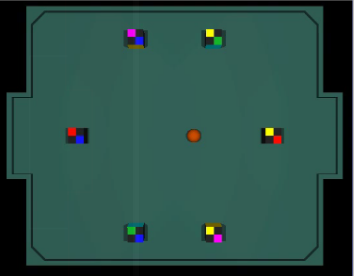
\includegraphics[width=0.6\textwidth]{figures/SimulatorWithoutButtons.png}
	\caption{Simulador da ITAndroids.}
	\label{fig:simulator}
\end{figure}


Com isso, é possivel ter uma aproximação do comportamento do time em um jogo real. Dado que o simulador é desenvolvido pela própria equipe, é possível adicionar situações especiais de jogo, além de se adicionar condições de paradas específicas para o que se deseja testar. Essas funcionalidades são muito importantes para a criação de situações específicas de jogo e, consequentemente, de funções de custo mais rápidas e otimizadas, o que garante uma convergência mais rápida de determinados parâmetros.

Além disso, o simulador também tem um modo de funcionar que é o chamado: modo acelerado. Normalmente, o código tem algumas funções para esperar um determinado tempo, com o objetivo de fazer que ele execute em tempo real (se ele não tivesse, a física seria muito rápida). Porém, no modo acelerado, esses tempos ociosos são removidos e a comunicação com o código principal funciona de forma assíncrona, o que garante uma velocidade de executação e simulação muito mais rápida, chegando a ser até dez vezes mais rápida que o modo de execução normal. Por essas razões, o modo acelerado é fundamental para garantir que a função de custo a ser desenvolvida seja mais eficiente e veloz.

\subsection{Univector Field}

O Univector Field é o planejamento de trajetórias usado pela equipe. O problema a ser resolvido é: como chegar de um ponto inicial à um ponto destino dentro do campo, desviando de obstáculos e considerando as limitações de controle e físicas do robô. Não será detalhado o funcionamento completo do algoritmo do Univector Field, já que isso pode ser visto em \cite{univector}.

Entretando, será descrito o que cada constante do algoritmo faz e uma descrição prática de como ela influencia na trajetória calculada, de modo a entender os resultados obtidos na otimização. Tem-se as seguinte constantes a serem otimizadas:
\begin{enumerate}
\item de: É o dobro de distância entre os centros de rotação do Univector Field. Na prática, quanto maior o seu valor, menos preciso o robô é em chegar em seu alvo. Se o seu valor for muito pequeno, o agente pode ficar preso em um mínimo local e nunca chegar em seu objetivo.
\item Kr: Define o quanto de rotação o campo gerado terá apontando para o seu alvo. Valores muito altos nessa constantes podem exigir que o robô faça curvas mais abruptas do que é possível e valores muito baixo farão que o robô faça curvas com raio muito grande, demorando mais a chegar no ponto desejado.
\item sigma: Parâmetro que define o tamanho do campo de repulsão gaussiano que o robô sofre de um obstáculo. Quanto maior o valor dessa constante, maior a repulsão do obstáculo.
\item dmin: A distância que o robô deve estar do obstáculo para o seu campo ser considerado infinito. Esse valor serve para garantir que o agente não colida com um obstáculo e deve ser otimizado para garantir que, se o robô se aproximar demais de um obstáculo, que ele seja repelido imediatamente e com muita intensidade.
\item K0: O parâmetro de predição de velocidade de obstáculos. É basicamente uma constante que é multiplicada pela velocidade do obstáculo para se calcular qual posição ele estará quando o agente chegar no objetivo. Único parâmetro que trata de obstáculos em movimento.
\item sigmaLine: Mesmo que o parâmetro sigma só que para as paredes do campo. As paredes são tratadas como um obstáculo especial já que, enquanto um obstáculo normal é um ponto, uma parede é uma reta.
\item dminLine:  O mesmo que a constante dmin só que para as paredes.
\end{enumerate}

O Univector Field é integrado com a interface de depuração da equipe, o que ajuda, qualitativamente, a verificar o quão otimizado é uma determinada trajetória gerada pelo algoritmo. Isso faz com que seja simples e rápido fazer uma checagem manual para saber se as constantes que o algoritmo convergiu não são absurdas.

\begin{figure}[H]
	\centering
	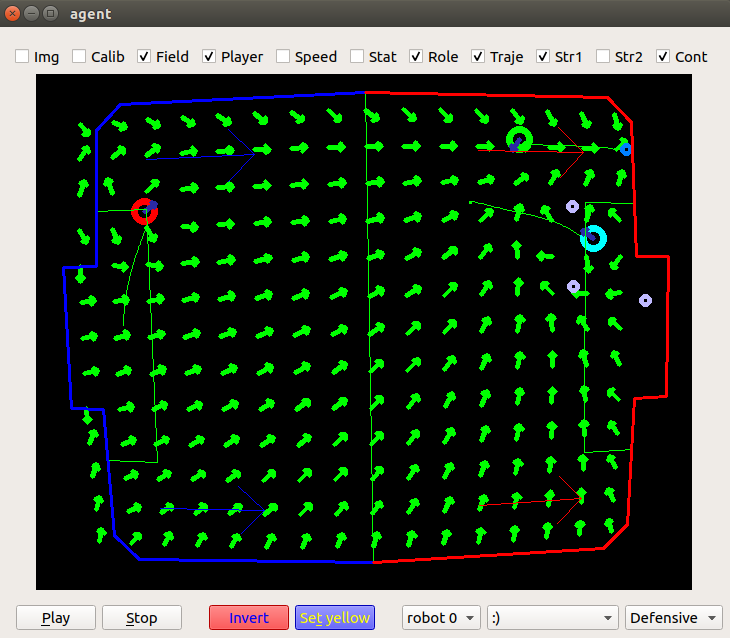
\includegraphics[width=0.83\textwidth]{figures/UnivectorFieldSimulatorDebugger.png}
	\caption{Interface gráfica para depuração da equipe}
	\label{fig:univector}
\end{figure}

Na Figura \ref{fig:univector}, é possível observar, em um determinado instante, as trajetórias calculadas para cada jogador e os vetores do campo do Univector Field para o jogador verde.


\section{Resultados Obtidos}
	\label{secao: resultados_obtidos}
    
Nessa seção, são apresentados os resultados obtidos na resolução do problema de otimização de parâmetros para robôs jogadores de futebol IEEE Very Small Size Soccer. Os resultados a seguir foram obtidos usando o simulador desenvolvido pela equipe.

\subsection{Função de Custo}

Aqui, será apresentado as situações de jogo escolhidas para serem simuladas para a otimização de parâmetros. É importante fixar que tais jogadas devem ser rápidas de serem executadas e realmente oferecerem resultados significantes para os parâmetros a serem otimizados. Cada situação escolhida deve ter uma função de custo associada que deve ser minimizada.
Para a otimização em questão, foi desenvolvido duas situações de jogo com objetivo de otimizar variáveis diferentes. Elas são executadas sequencialmente, ou seja, a segunda situação de jogo usará os resultados obtidos da primeira situação.

\subsubsection{Trajetórias Básicas}

Nesse primeiro caso, será tratado o problema de um só jogador no campo com o objetivo de apenas jogar a bola para frente. Nessa situação, o foco será otimizar os parâmetros mais simples do planejamento de trajetória, que são todos não relacionados ao desvio de oponentes, mas incluindo os parâmetros relativos à repulsão de paredes.

O jogador e a bola são postos em diversas posições fixas no campo. Em seguida o jogador deve se mover até a bola e chutá-la ou conduzi-la até o final do campo do oponente. Quando a bola chega no final do campo, marca-se o tempo que demorou para esse objetivo ser atingido e começa o teste novamente para a próxima posição predeterminada. Caso o objetivo não seja alcançado em 3 minutos no tempo de jogo (a simulação é executada no modo acelerado), termina-se a simulação imediatamente.

Dessa forma, calcula-se a função de custo de acordo com a seguinte equação:

$ F = tempoTotalDeTodasAsPosicoesRealizadas - numeroDePosicoesCompletadas. $
 
Nota-se que, de acordo com essa função fitness que deve ser minimizada, quanto menos tempo o agente completar todas a posições e quanto mais posições ele completar, melhor será o fitness calculado.

A Figura \ref{fig:sem_obstaculo_simulacao} mostra uma posição do jogador e da bola para essa situação de jogo.

\begin{figure}[H]
	\centering
	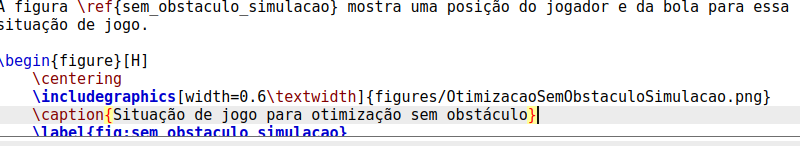
\includegraphics[width=0.6\textwidth]{figures/OtimizacaoSemObstaculoSimulacao.png}
	\caption{Situação de jogo para otimização de trajetória simples}
	\label{fig:sem_obstaculo_simulacao}
\end{figure}


\subsubsection{Desvio de Obstáculos}

Esse caso é bastante similar à situação anterior no sentido que usará a mesma função de custo. A diferença consiste no fato de que, nessa situação, será posto um obstáculo (um jogador aliado) na frente da bola, de modo a obrigar que o agente principal desvie do obstáculo e rapidamente retorne à trajetória original para conseguir chegar na bola.

Nessa situação, será otimizado apenas as variáveis relativas ao desvio de obstáculos. Está sendo assumido que os parâmetros relativos à repulsão de paredes e os de planejamento de trajetória básicos já estão otimizados e funcionais.

A Figura \ref{fig:com_obstaculo_simulacao} mostra uma posição do jogador, do obstáculo e da bola para essa situação de jogo. Percebe-se que o obstáculo está posicionado bem perto da bola, o que obriga o agente principal a fazer o desvio em sua trajetória. Nesse caso, o agente que vai tentar chegar na bola é o jogador rosa-azul, enquanto que os outros jogadores são obstáculos.

\begin{figure}[H]
	\centering
	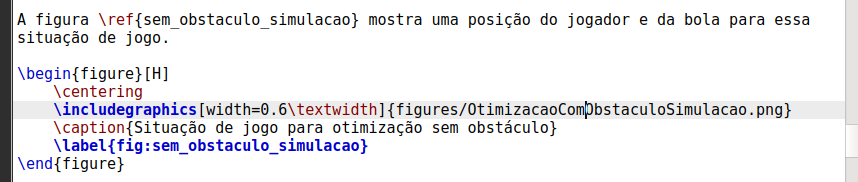
\includegraphics[width=0.6\textwidth]{figures/OtimizacaoComObstaculoSimulacao.png}
	\caption{Situação de jogo para otimização de desvio de obstáculos}
	\label{fig:com_obstaculo_simulacao}
\end{figure}


\subsection{Otimização}

Nessa secção, será apresentado os resultados obtidos ao executar o algoritmo de otimização CMA-ES com as funções de custo apresentadas anteriormente. Será mostrado e comentado como foi a convergência geral do algoritmo e dos parâmetros em cada caso.

\subsubsection{Trajetórias Básicas}

A Figura \ref{fig:fitness_trajetoria_basica} mostra a evolução do custo da população com o passar das iterações. Foi realizado uma interpolação polinomial de terceira ordem para os resultados obtidos, de modo a melhor visualizar os efeitos da convergência. A interpolação pode ser visualizada pela linha vermelha, enquanto que os pontos `X’ representam o resultado de cada iteração em específico.

\begin{figure}[H]
	\centering
	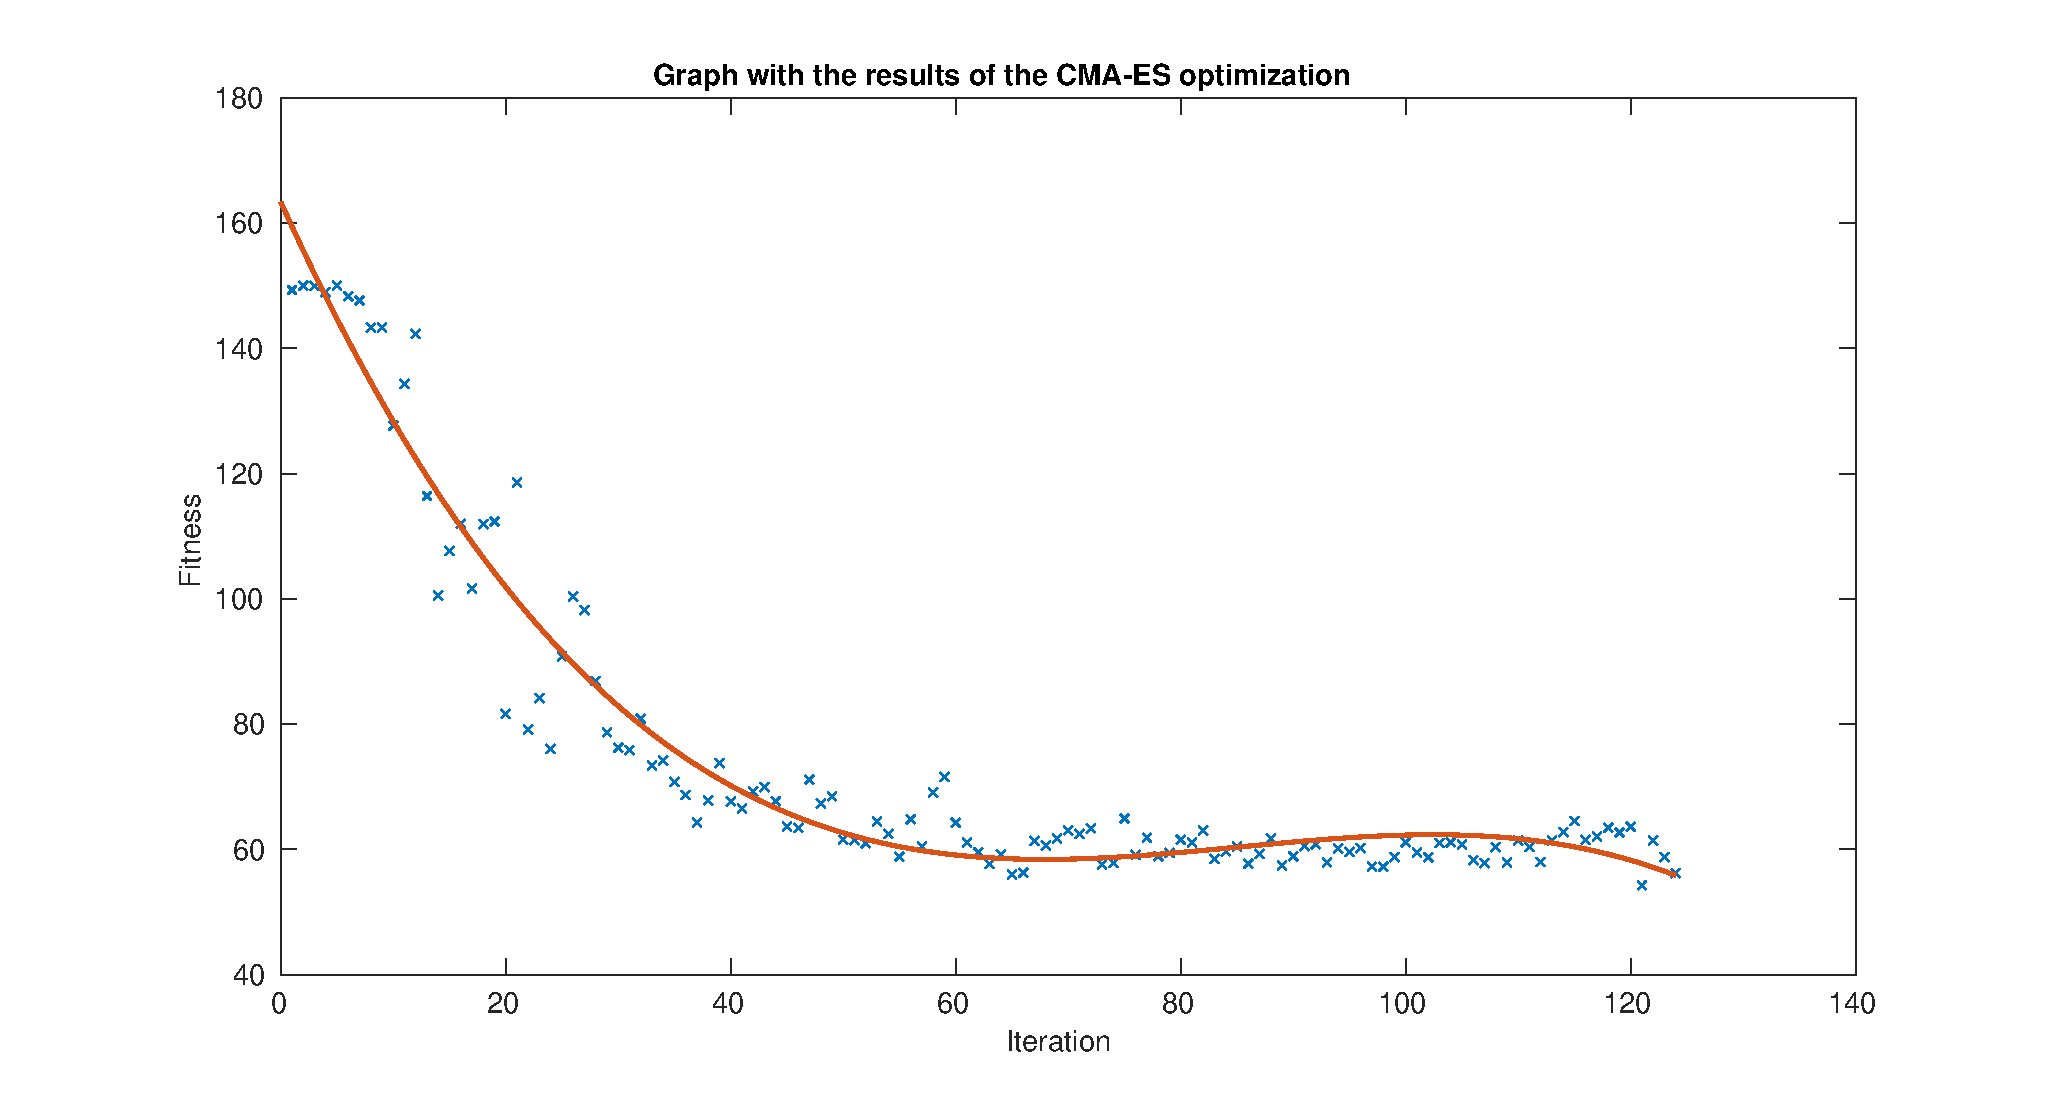
\includegraphics[width=1.0\textwidth]{figures/CMA-ES_Fitness_Results.eps}
	\caption{Fitness Cost em função do número de iterações}
	\label{fig:fitness_trajetoria_basica}
\end{figure}

De acordo com a Figura \ref{fig:fitness_trajetoria_basica}, nota-se que, de fato, o algoritmo de otimização tende a reduzir o valor do Fitness Cost à medida que o número de iterações aumenta. Em torno de 60 iterações porém, o algoritmo já converge para um valor e não acontece melhoras significativas a partir desse momento.

Na Figura \ref{fig:convergencia_total_trajetoria_basica} temos a convergência total dos parâmetros normalizada. A normalização foi feita em cada parâmetro separadamente e depois foi calculado a média desses resultados para cada iteração.

\begin{figure}[H]
	\centering
	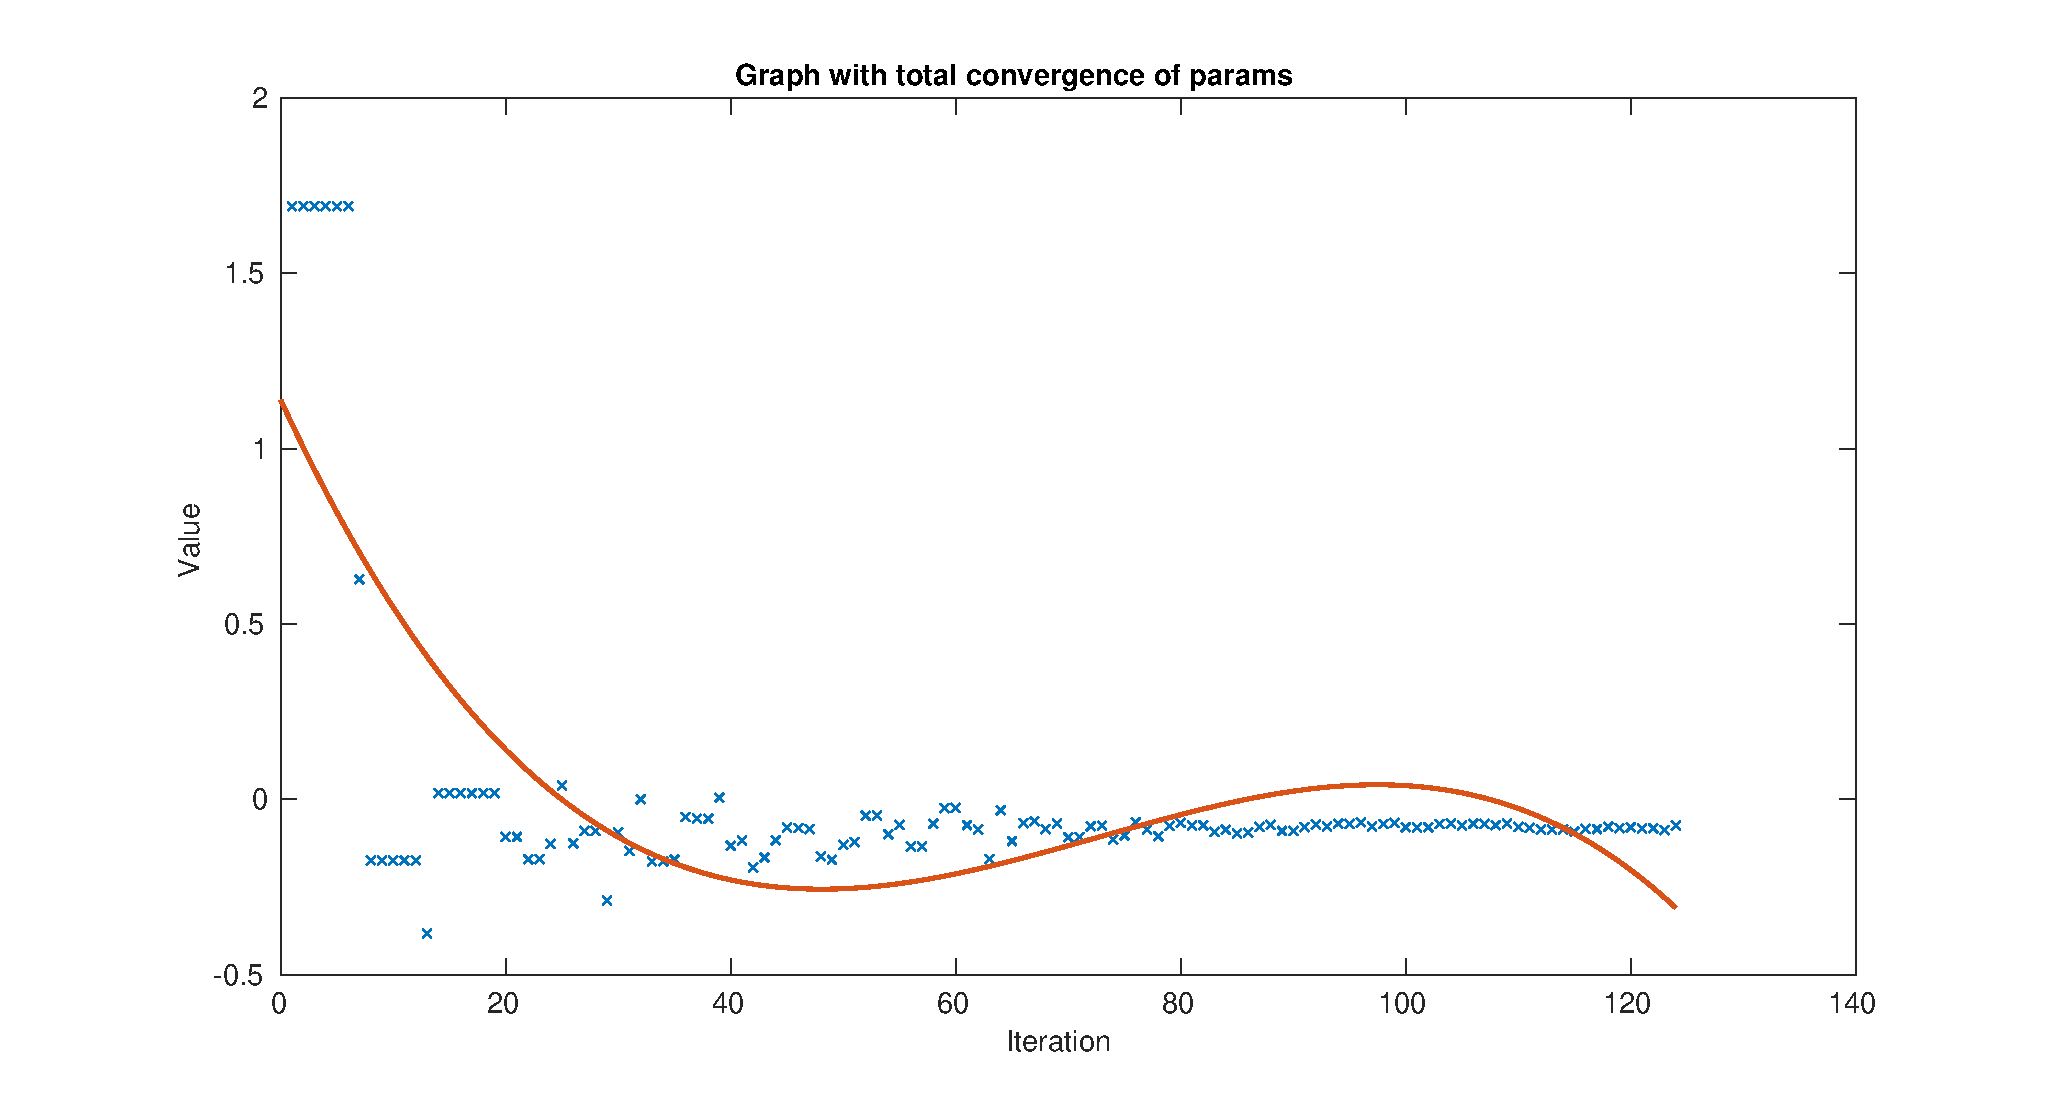
\includegraphics[width=1.0\textwidth]{figures/CMA-ES_Total_parameter_convergence.eps}
	\caption{Convergência total dos parâmetros em função do número de iterações}
	\label{fig:convergencia_total_trajetoria_basica}
\end{figure}

Tanto a Figura \ref{fig:convergencia_total_trajetoria_basica}, quanto a Figura \ref{fig:fitness_trajetoria_basica} confirmam uma correta convergência do algoritmo, que converge em torno de 100 iterações.

\subsubsection{Desvio de Obstáculos}

A Figura \ref{fig:fitness_trajetoria_basica_ally} mostra a evolução do custo em função de uma determinada iteração do algoritmo para a otimização de desvio de obstáculos. Nota-se que os pontos nessa figura são mais esparsos que o da Figura \ref{fig:fitness_trajetoria_basica}, o que é esperado, já que a otimização de desvio de obstáculos é mais complexa que a de trajetórias básicas.

\begin{figure}[H]
	\centering
	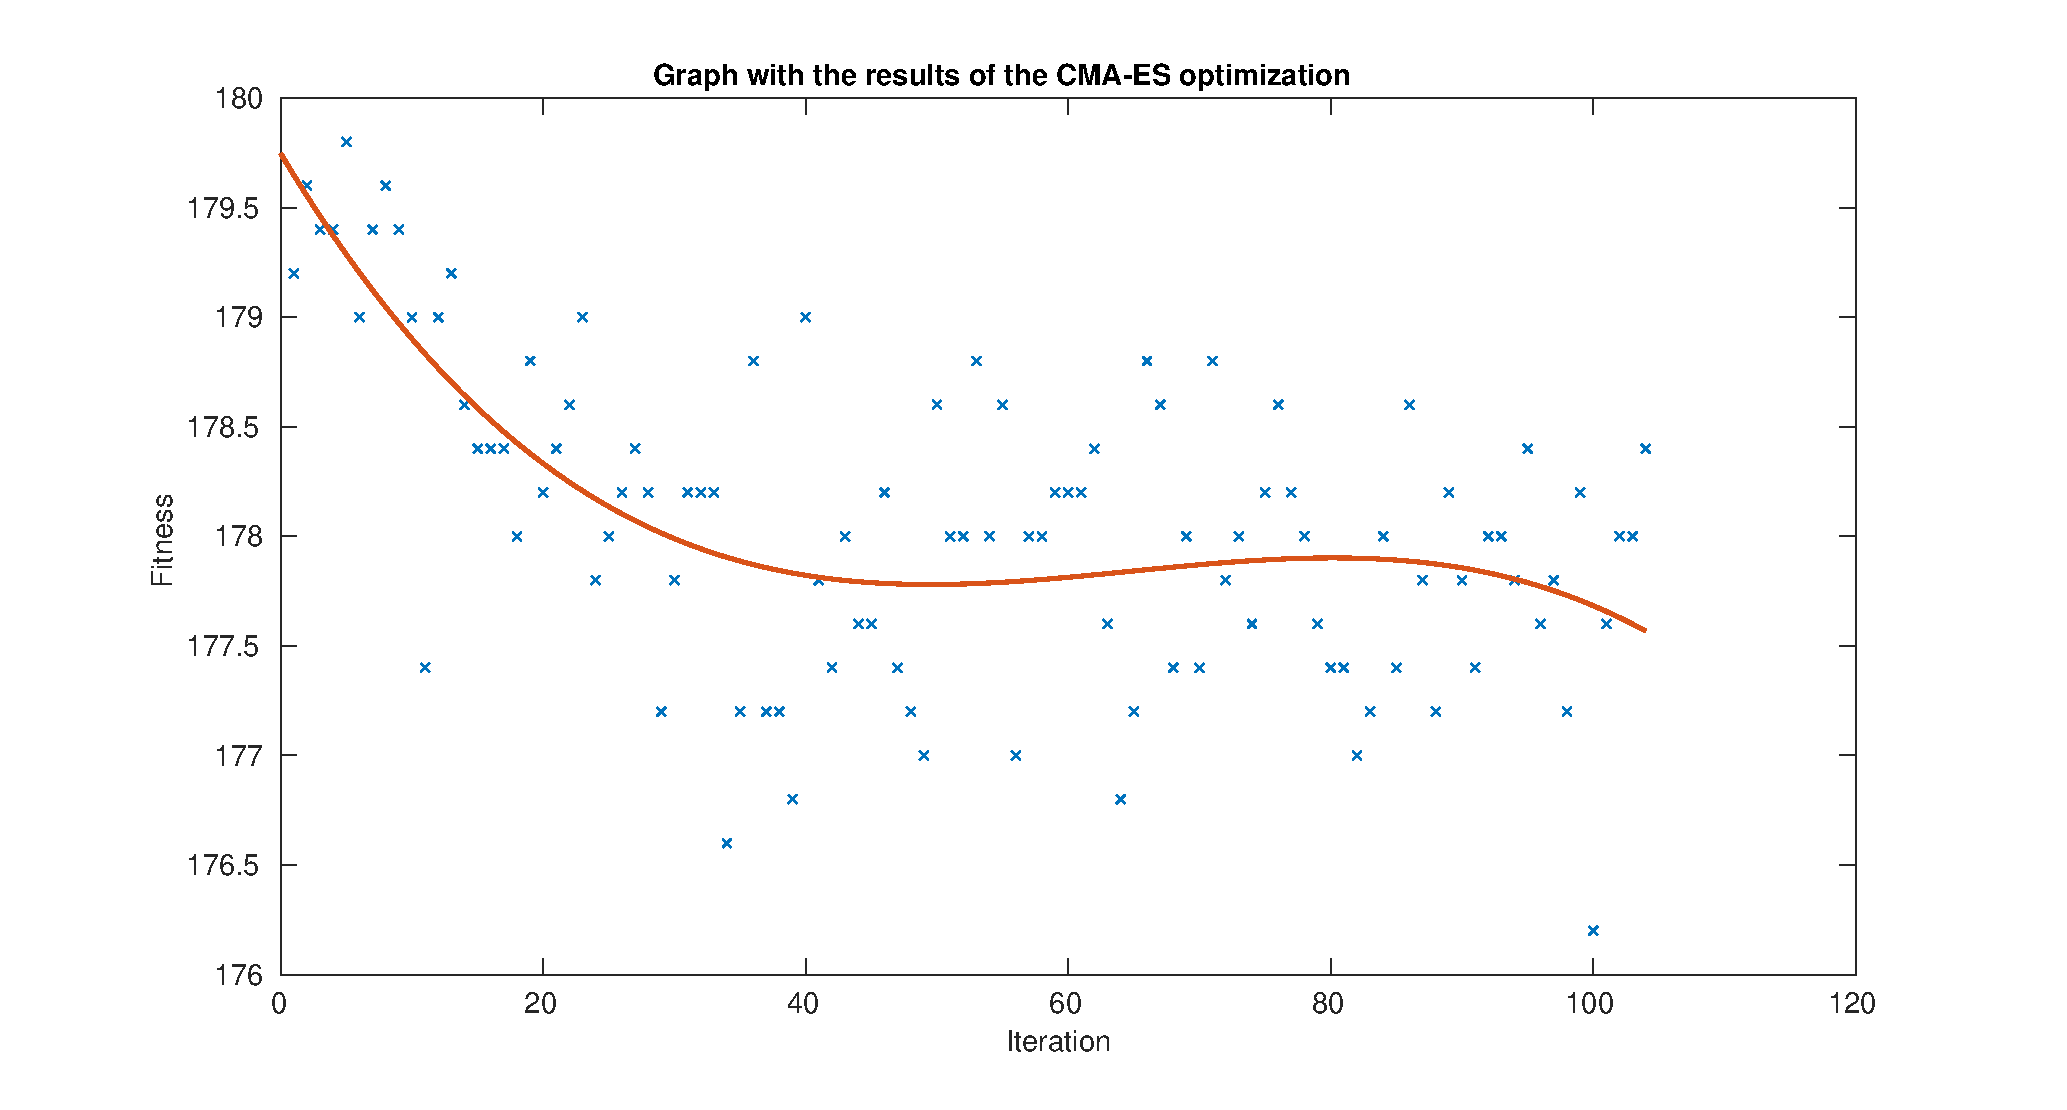
\includegraphics[width=1.0\textwidth]{figures/CMA-ES_Fitness_Results_ally.eps}
	\caption{Fitness Cost em função do número de iterações}
	\label{fig:fitness_trajetoria_basica_ally}
\end{figure}

Na Figura \ref{fig:convergencia_total_trajetoria_basica_ally} temos a convergência total dos parâmetros normalizada. A normalização foi feita em cada parâmetro separadamente e depois foi calculado a média desses resultados para cada iteração.

\begin{figure}[H]
	\centering
	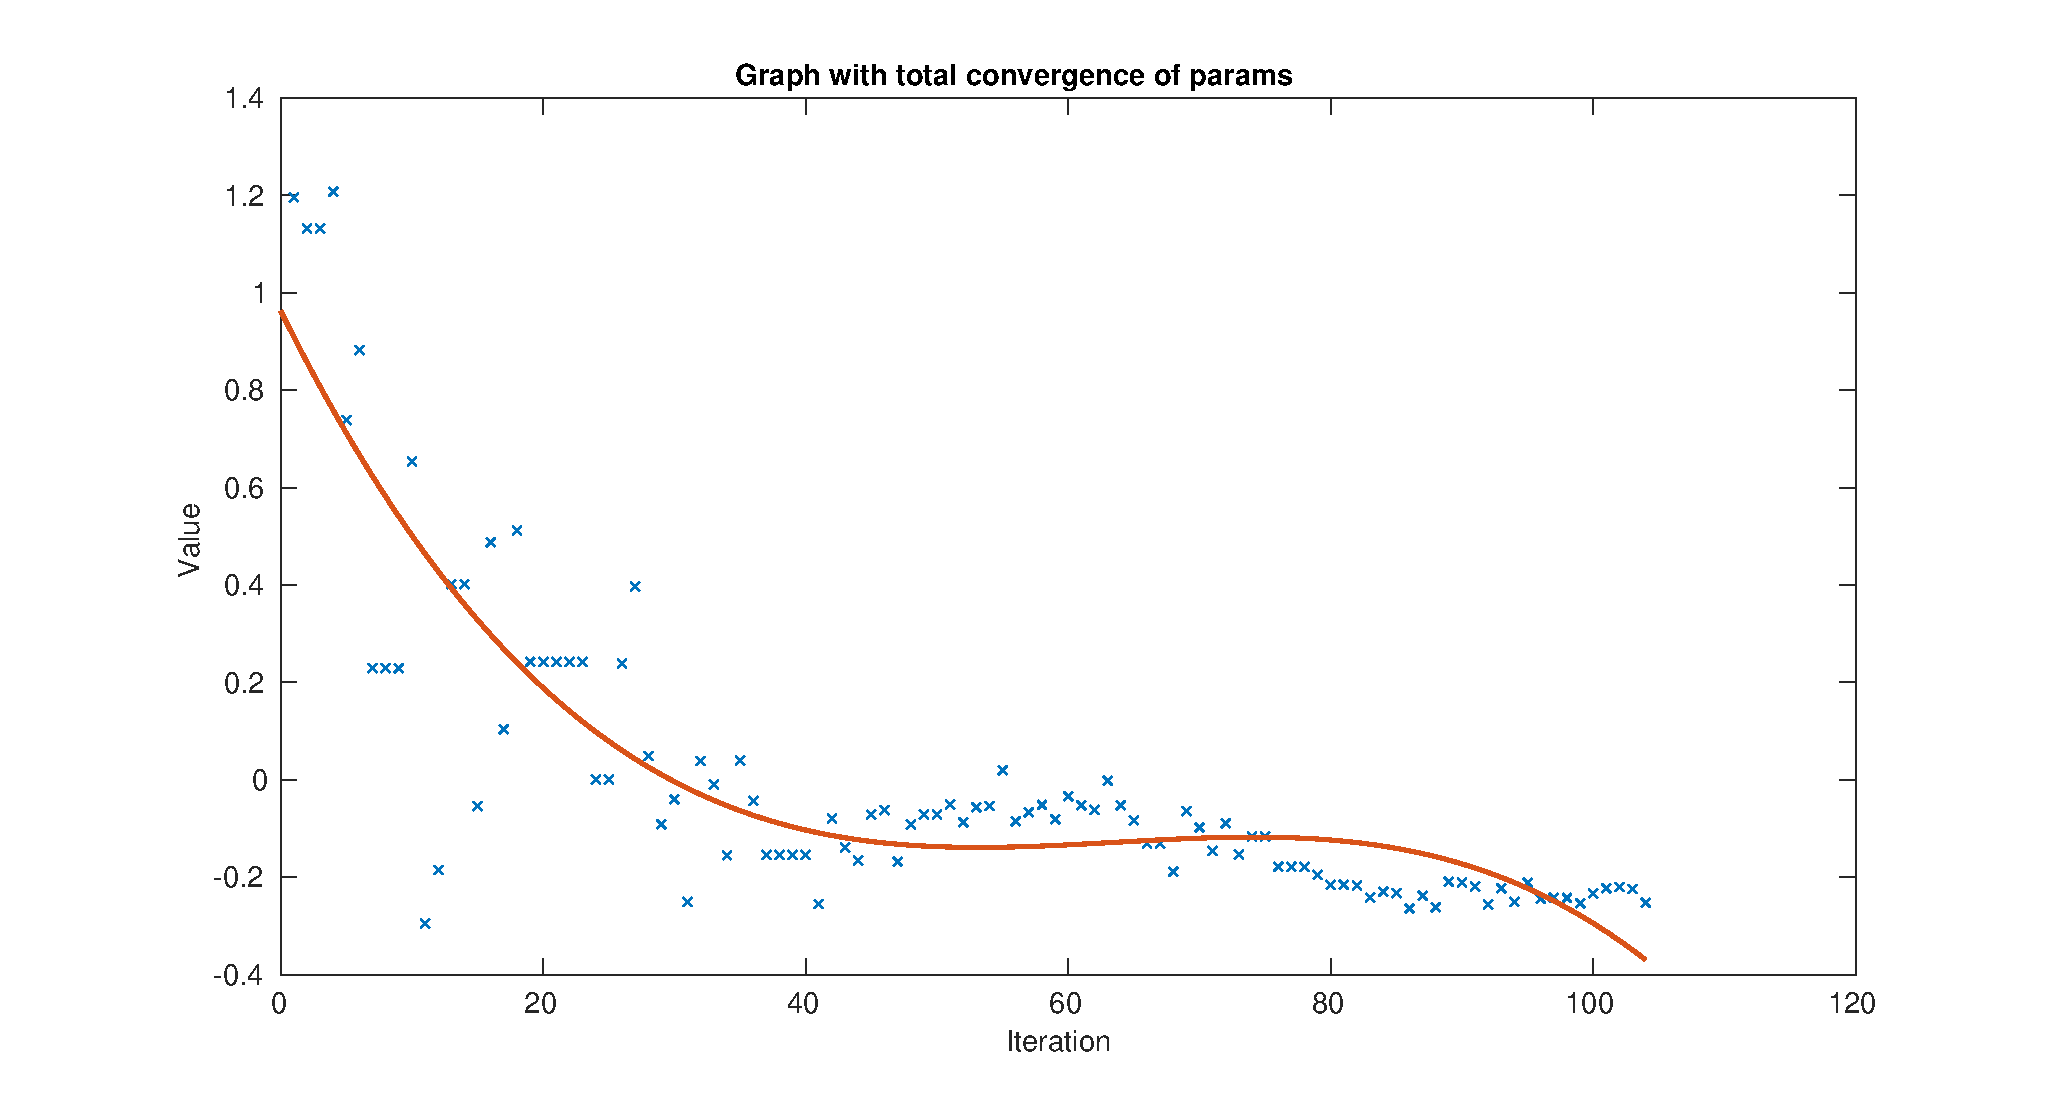
\includegraphics[width=1.0\textwidth]{figures/CMA-ES_Total_parameter_convergence_ally.eps}
	\caption{Convergência total dos parâmetros em função do número de iterações}
	\label{fig:convergencia_total_trajetoria_basica_ally}
\end{figure}

Tanto a Figura \ref{fig:convergencia_total_trajetoria_basica_ally}, quanto a Figura \ref{fig:fitness_trajetoria_basica_ally} confirmam uma correta convergência do algoritmo, que converge em torno de 100 iterações.

\section{Conclusões}

O projeto de Iniciação Científica apresentou bons resultados, especialmente quanto à vitória da equipe do ITA na competição CBR 2018, rendendo o primeiro lugar à equipe, na primeira vez da história, dentre mais de 25 equipes participantes de toda América Latina.

Do ponto de vista técnico, o uso do algoritmo Covariance Matrix Adaptation Evolution Strategy se mostrou factível e funcional para otimização de parâmetros para o planejamento de trajetórias, com resultados demonstrados em partidas oficiais.

Com a estrutura de otimização implementada para a equipe, próximos passos incluem utilizar esse algoritmo para outras áreas do código, como otimização na tomada de decisão do time de robôs.

\section{Agradecimentos}

\begin{itemize}
\item Ao CNPq, pelo apoio financeiro e motivacional.
\item À ITAndroids, equipe que representa o ITA na competição da LARC/CBR, pela ideia do projeto, pela disponibilidade do robô real para implementação e oportunidade de aplicação dos métodos estudados.
\item Ao professor doutor Celso Massaki Hirata, meu orientador, e ao professor doutor Marcos Ricardo de Omena Máximo, co-orientador, ambos da Divisão da Ciência da Computação do ITA, pelo apoio nos estudos e no desenvolvimento do projeto.

\end{itemize}

\section{Bibliografia}

\printbibliography


\end{document}